\documentclass[12pt]{article}

\usepackage{graphicx}
\usepackage{amsfonts, amsmath, amsthm, amssymb}
%\usepackage{wrapfig}
\usepackage{indentfirst}
\usepackage{hyperref}
\hypersetup{
    colorlinks=true,
    linkcolor=blue,
    filecolor=magenta,      
    urlcolor=cyan,
}

\urlstyle{same}

\begin{document}
\title{HAPIEST User Manual} 
\date{}
\maketitle
\thispagestyle{empty}
\newpage
\tableofcontents
\thispagestyle{empty}
\newpage
\setcounter{page}{1}

\section{HAPIEST}
HITRAN Application Programming Interface and Efficient Spectroscopic Tools (HAPIEST) is a GUI for the HITRAN Application Programming Interface\footnote{R.V. Kochanov, I.E. Gordon, L.S. Rothman, P. Wcislo, C. Hill, J.S. Wilzewski, HITRAN Application Programming Interface (HAPI): A comprehensive approach to working with spectroscopic data, J. Quant. Spectrosc. Radiat. Transfer 177, 15-30 (2016) DOI: \href{https://doi.org/10.1016/j.jqsrt.2016.03.005}{10.1016/j.jqsrt.2016.03.005} } (HAPI). HAPIEST's development began at SUNY Oswego in a software engineering course by students Benji Caro, Joshua Karns, Dominik Lohmann, Wyatt Matt, Ethan Messer, and Michael Sova, and in conjunction with Dr. Iouli Gordon and Dr. Roman Kochanov of the Harvard-Smithsonian Center for Astrophysics and under advisement of SUNY Oswego professor Bastian Tenbergen and SUNY Oswego Professors and Head of Physics Department Shashi Kanbur.

\subsection{Program Overview}
The goal of HAPIEST is to simplify the use of the HAPI for all users. Currently, HAPI requires some knowledge of Python and use of the command line. HAPIEST retains as much of the functionality HAPI as is possible in a simple GUI, while making it easier for the user to access and use HITRAN data. HAPIEST currently allows users the capability to fetch/download and locally store data from the HITRAN database, edit local data, and also to generate and plot spectral functions. In it's current form, the HAPIEST interface is split into three windows; one window for data management and editing, and two windows for graphing/graph display.

\subsection{Installation}
HAPIEST is available to follow and download on our \href{https://github.com/hitranonline/hapiest}{GitHub} for the latest pre-release version. A 'display' distribution is also available on \href{https://github.com/hitranonline/hapiest/releases}{GitHub} for Windows, and will be coming to Linux and Mac.

\newpage

\section{Molecules Tab}
The molecules tab, shown in Fig.~\ref{fig:molecules}, provides reference for the available molecules and also reference ID's for each molecule.
\begin{figure}[h]
\centering
    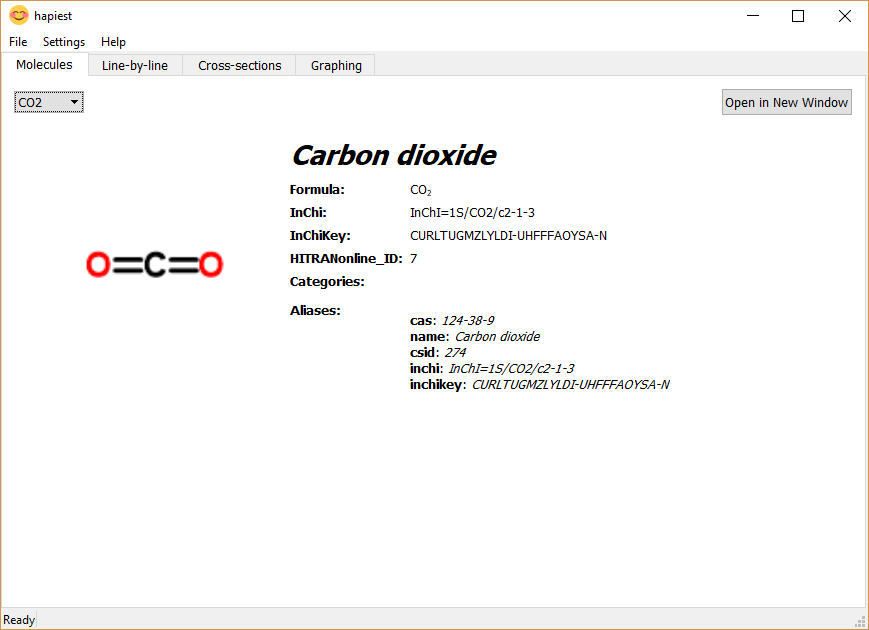
\includegraphics[scale=1]{hapiest_molecules.png}
\caption{Example display of Carbon Dioxide}
\label{fig:molecules}
\end{figure}


\section{Line-by-line Tab}
The Line-by-line tab allows the user to download data from HITRAN onto their local disk for the available molecules and their supported isotopologues. Furthermore, the user can select from the Parameter Groups list and Parameters list to download more specific data. This window is the users primary method of obtaining data.
\begin{figure}[h]
\centering
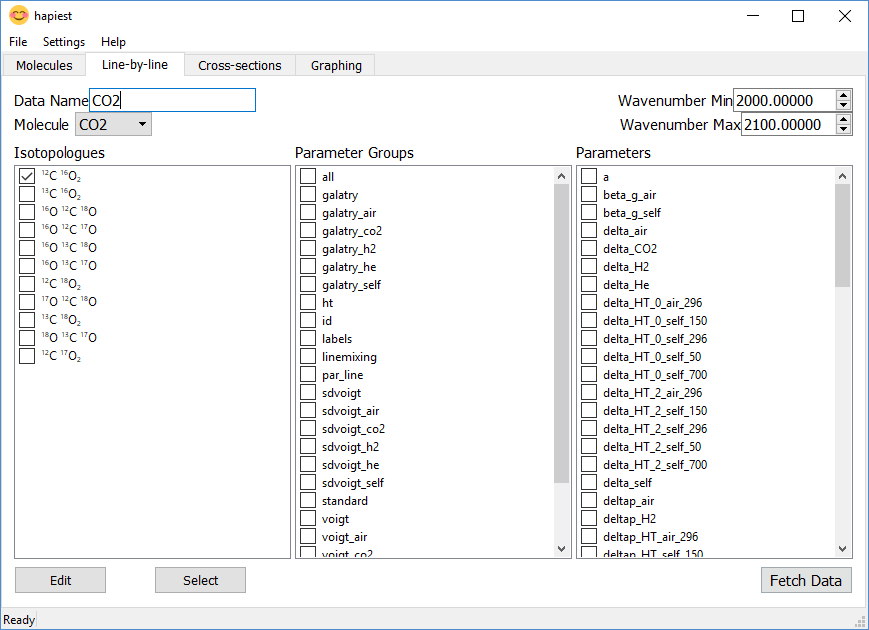
\includegraphics[scale = 0.6]{hapiest_line_by_line.png}
\caption{Line-by-line tab filled out to fetch data for CO2}
\label{fig:line-by-line}
\end{figure}
\addcontentsline{toc}{subsubsection}{Fetch Dictionary}

\newpage
\subsection*{Line-by-line Dictionary}
\begin{itemize}
\item Data Name - Local file name of data being downloaded.
\item Molecule - List of molecules to select which Isotopologues to fetch data for, updates the Isotopologues list when a molecule is selected.
\item Wave Number Min - Lower threshold to fetch data (from).
\item Wave Number Max - Upper threshold to fetch data (to).
\item Isotopologues - List of Isotopologues for the selected molecule. This is what you are fetching data for.
\item Parameter Groups - List containing groups of spectral line parameters.
\item Parameters - List of individual spectral line parameters to fetch for selected isotopologues.
\item Edit - Opens the Edit window.
\item Select - Opens the Select window.
\end{itemize}
\newpage

\subsection{Edit}
The Edit tab, shown in Fig.~\ref{fig:edit}, allows users to view and edit local data that has been downloaded through HAPIEST. It offers a table view of all parameters and values, and can be saved to disk.
\begin{figure}[h]
\centering
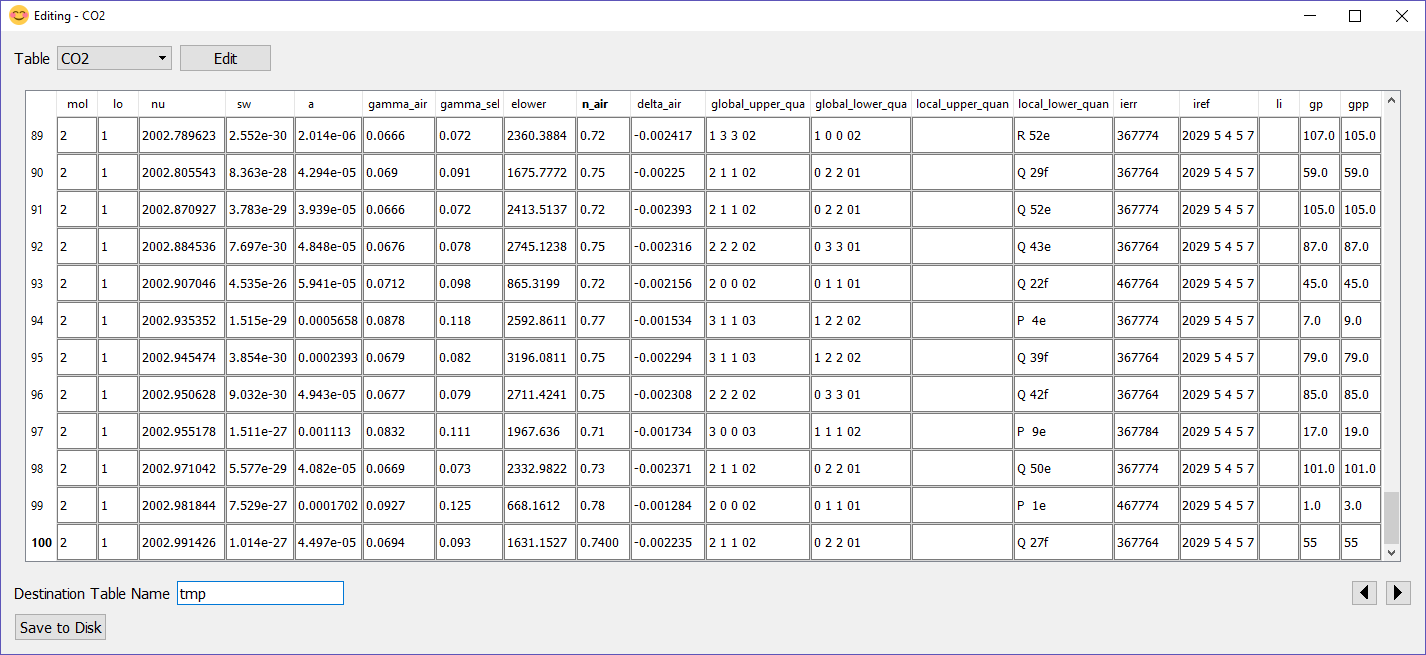
\includegraphics[scale = 0.5]{hapiest_edit.png}
\caption{Generated table of downloaded parameters}
\label{fig:edit}
\end{figure}
\addcontentsline{toc}{subsubsection}{Edit Dictionary}

\subsubsection*{Edit Dictionary}
\begin{itemize}
\item Table - List of HITRAN data files.
\item Edit - Button that populates table containing information in the data file.
\item Destination Table Name - Name of local file upon saving.
\item (Left and Right Arrows) - Select between pages of data.
\item Save to Disk - Button that saves the  current table to disk.
\end{itemize}
\newpage


\subsection{Select}
The Select tab, shown in Fig.~\ref{fig:select}, is dedicated to the select function available in HAPI and allows users a more advanced fetch.
\begin{figure}[h]
\centering
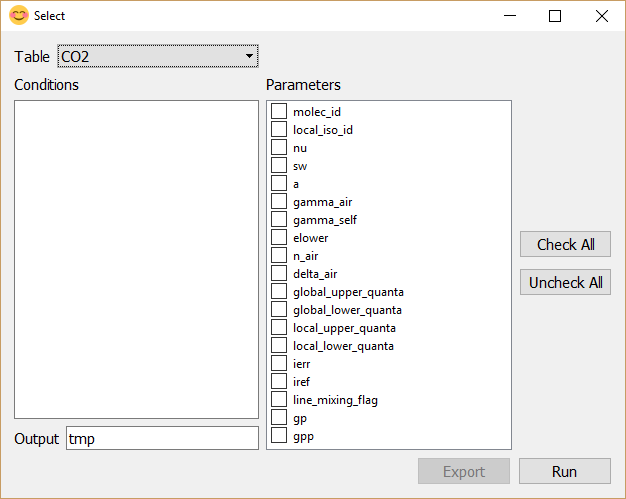
\includegraphics[scale = 0.6]{select_window.png}
\caption{Page resulting from Select tab}
\label{fig:select}
\end{figure}

\section{Cross-Sections Tab}
-

\section{Graphing Tab}
In the Graphing tab, shown in Fig.~\ref{fig:graphing}, the user is given a list of parameter fields to populate in order to create the specific graph they need for each graph type (Absorption Coefficient; Absorption, Transmittance, and Radiance Spectra graphs). Multiple plots of the same type may be displayed together on the same graph.
\begin{figure}[h]
\centering
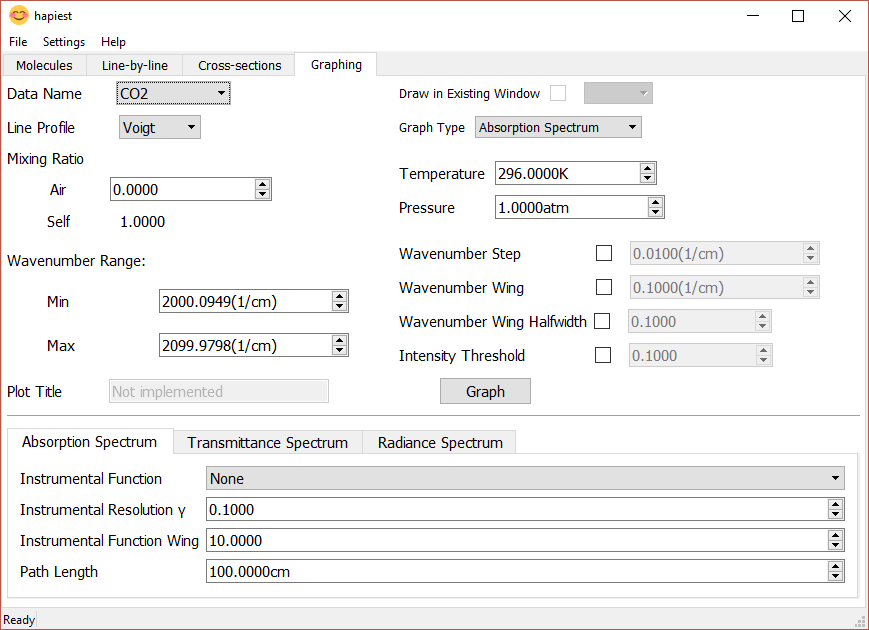
\includegraphics[scale = 0.6]{hapiest_graphing.png}
\caption{Example of Graphing tab}
\label{fig:graphing}
\end{figure}

\addcontentsline{toc}{subsubsection}{Graphing Dictionary}
\subsection*{Graphing Dictionary}
\begin{itemize}
\item Data Name - Data file used to calculate spectra for graphing.
\item Draw in Existing Window - Checkbox to enable multiple plots on the same graph for the same Line Profiles. List of graph windows open to plot to.
\item Line Profile - Line profile (lineshape) type to use in the spectra calculation..
\item Graph Type - Type of the graph to plot: dependent on the spectra type (i.e. absorption, transmittance, etc...).
\item Mixing Ratio - Volume mixing ratio of air in the modeled mixture.
\item Temperature - Temperature (Kelvin) of the modeled gas mixture.
\item Pressure - Total pressure (in atmospheres) of the modeled gas mixture.
\item Wavenumber Range - Spectral range to be used in the simulation (in wavenumbers)
\item Wavenumber Step - Wavenumber step to be used in the simulation.
\item Wavenumber Wing - Absolute size of the wing (in wavenumbers) at which line profile is not zero.
\item Wavenumber Wing Halfwidth - Relative of the size of the wing (in line halfwidths) at which line profile is not zero.
\item Intensity Threshold - Minimum value of the line intensity to consider in the spectra calculation.
\item Plot Title - Title of the plot.
\item Graph - Button that creates a plot according to selected parameters.
\end{itemize}

\section{Graph Window}
Graphs are displayed in this window, an example is shown in Fig.~\ref{fig:graph_tab}. There is an option in the graphing tab to display multiple graphs in the same window (see Fig.~\ref{fig:graphing}). 

\subsection{User Interactivity}
Inside the graph display windows, the user has options to zoom in on the graph, reset view, choose between log/linear plotting, and save the graph in popular file formats. The menu bar contains three items: File is used for saving graphs to local disk; View contains options to change the view of the graph; and Scale allows the user to change between linear, base 10 log, and natural log plots for both the X and Y-axis. 

\addcontentsline{toc}{subsubsection}{Box Zoom}
\subsubsection*{Box Zoom}
To box zoom  (see Fig.~\ref{fig:graph_tab}), hold the left mouse button down and drag across the area you want to zoom in on, and release. In order to reset the graph view, click View in the menu and then click Fit.
\begin{figure}[h]
\centering
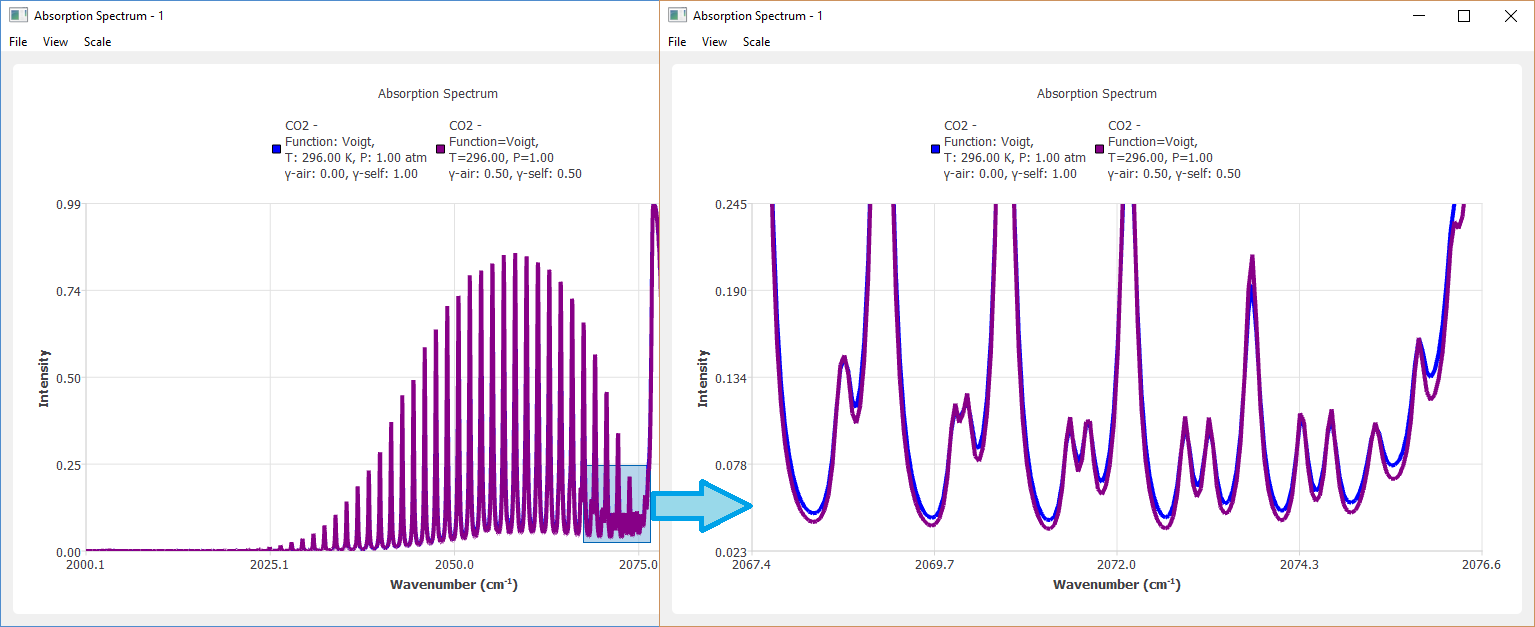
\includegraphics[scale = 0.4]{GraphBoxZoomBoth.png}
\caption{Example of a box zoom of a spectrum. The blue box is highlighted, and the new plot is given in the same window by using the multiple graphing functionality}
\label{fig:graph_tab}
\end{figure}

\subsubsection*{View}
In the graph window and under View in the menu, there are options to alter the viewing window of the graph. Clicking on Fit resets the graphing window to the original view of the graph, while clicking on exact gives the user the option to specifically enter the on-axis values they want to highlight/display.

\addcontentsline{toc}{subsubsection}{Save Features}
\subsubsection*{Save Features}
\begin{figure}[h]
\begin{minipage}[c]{0.3\textwidth}
\centering
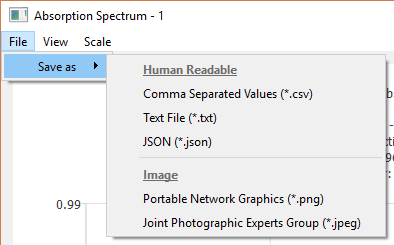
\includegraphics[scale = 0.5]{GraphSave.png}
\caption{Sequence of steps to generate plots}
\label{fig:save}
\end{minipage}
\hfill\vline\hfill
\begin{minipage}[c]{0.6\textwidth}
Under File in the menu bar, there are options to save graphs in image formats PNG and JPEG, or  text based as Comma Separated Values (CSV), Text File (TXT), or in JSON format (shown in Fig.~\ref{fig:save}).
\end{minipage}
\end{figure}
\newpage
\section{How to Use}

\subsection{Fetching Data}
In order to plot/graph data, the user needs to first download data from the HITRAN database. This can be done in HAPIEST or using HAPI. To do so in HAPIEST, follow the instructions below, along with Fig.~\ref{fig:how_to_fetch}.

\begin{figure}[h]
\centering
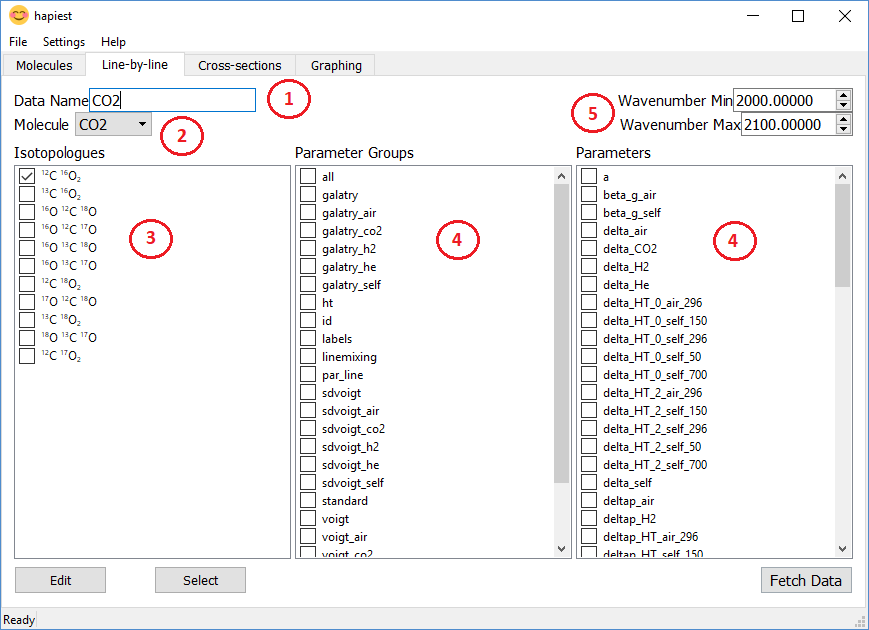
\includegraphics[scale = 0.6]{hapiest_line_by_line_guide.png}
\caption{Sequence of steps to fetch data}
\label{fig:how_to_fetch}
\end{figure}

\begin{enumerate}
\item Edit data name to change the name of the file downloaded upon fetching.
\item Select the molecule to update the Isotopologues list.
\item Select the Isotopologues you want to download data for.
\item Select from the Parameter Groups and Parameters list to download further data for the selected Isotopologues.
\item Edit the Wave Number Min and Max values to refine your download (Smaller ranges are faster to fetch and take up less space).
\end{enumerate}

\subsection{Graphing Data}
Once you have data on your system, you can then go to the Graphing Tab to produce a graph. Follow the instructions below, along with Fig.~\ref{fig:how_to_graph}
\begin{figure}[h]
\centering
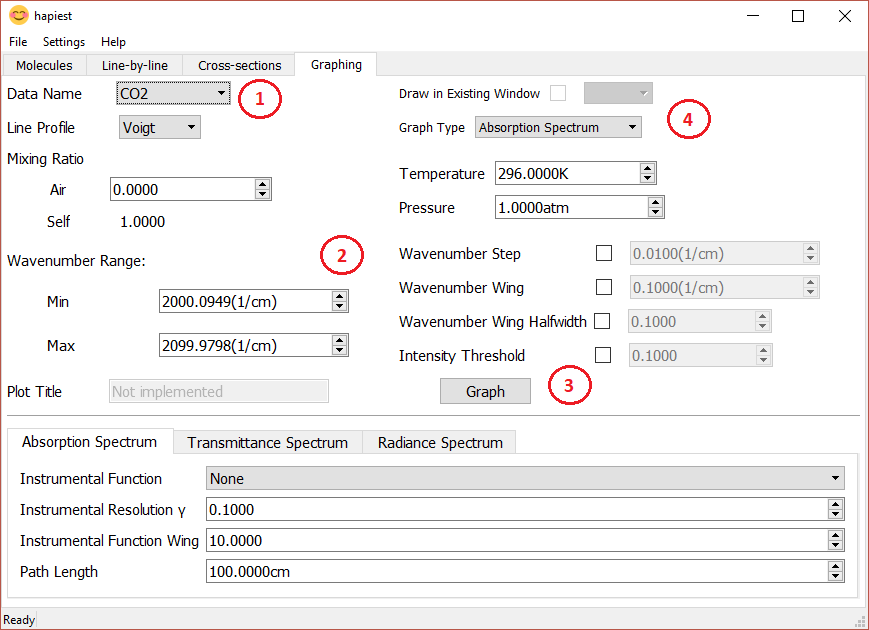
\includegraphics[scale = 0.6]{hapiest_graphing_guide}
\caption{Sequence of steps to generate plots}
\label{fig:how_to_graph}
\end{figure}
\begin{enumerate}
\item In the Data Name list, select the data file you want to use to create a plot.
%\item Skip Draw in Existing Window for now, and select the parameters of the plot.
\item Select the parameters used for the plot.
\item Clicking the Graph button will generate another window to display the graph.
\item Now, if you want to plot another graph of the same type in/with a previous plot, check the Draw in Existing Window check box and select the compatible window in the drop-down list.
\end{enumerate}

\end{document}
